\documentclass{article}

\usepackage{graphicx}
\usepackage{tikz}
\usepackage{tikzsymbols}
\usetikzlibrary{calc,patterns,shapes.geometric}
\pagestyle{empty}
\usepackage[margin=0pt]{geometry}
\geometry{papersize={14in,12in}}

\def\centerarc[#1](#2)(#3:#4:#5){\draw[#1] ($(#2)+({#5*cos(#3)},{#5*sin(#3)})$) arc (#3:#4:#5);}

\begin{document}
	\begin{figure}
		\centering
		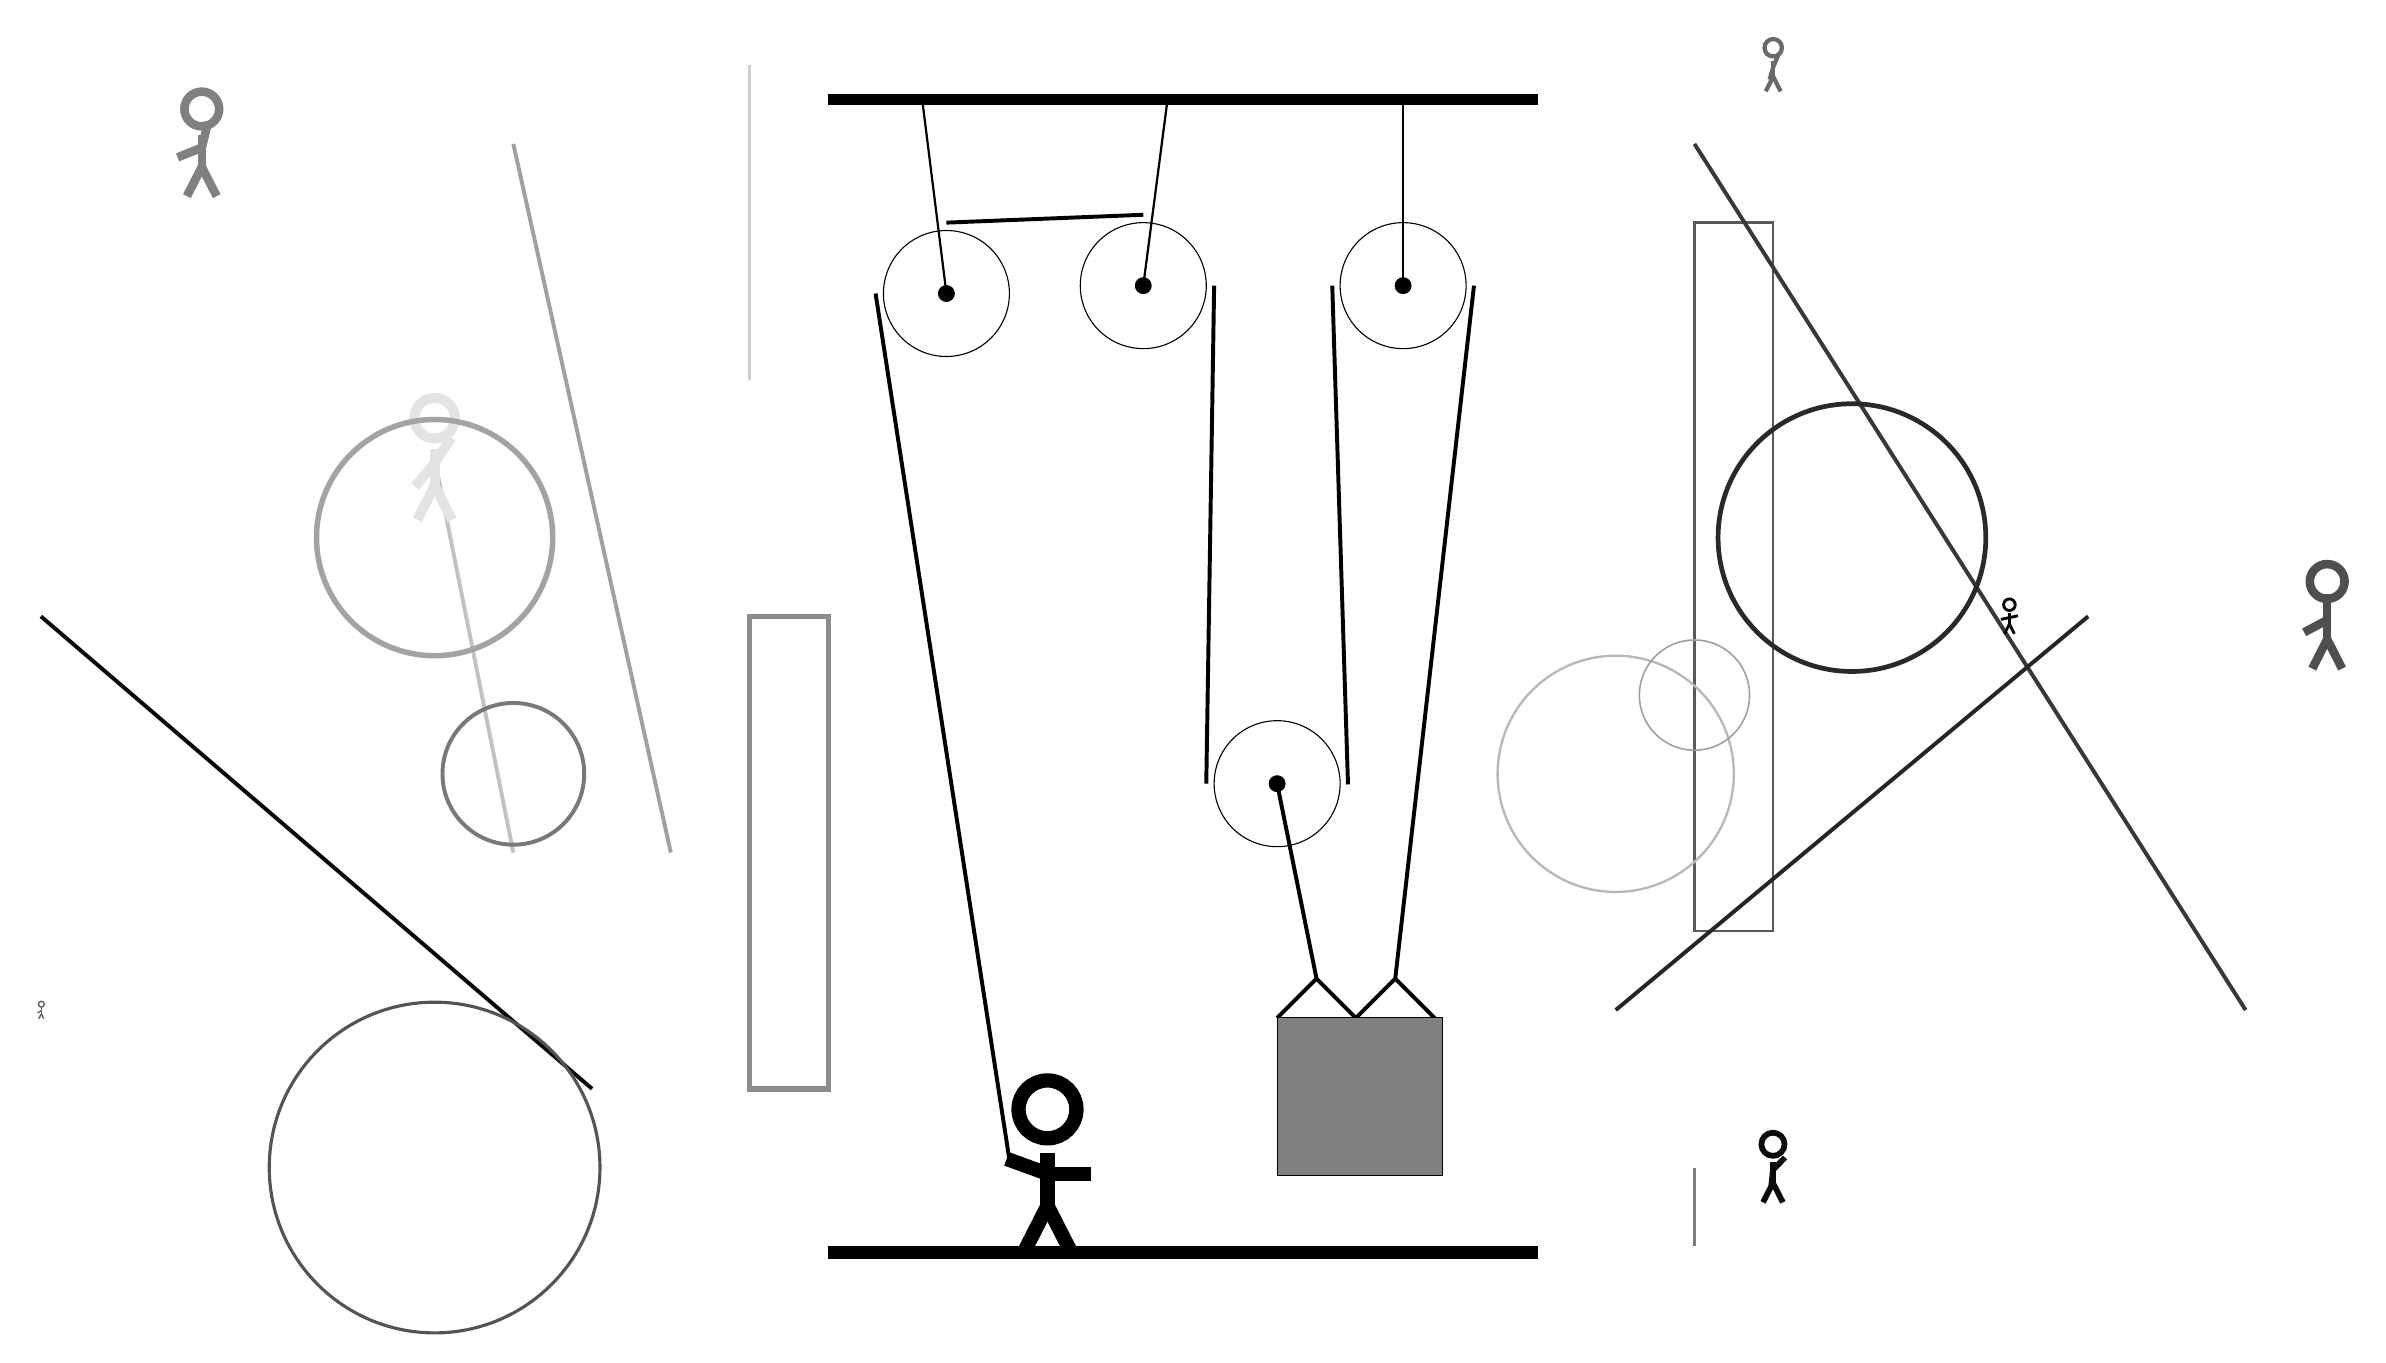
\begin{tikzpicture}
			%%%%% START %%%%%
			
			\draw[fill=black] (-3, 11.5) rectangle (6, 11.625);
			
			\draw (1, 9.2) circle (0.8);
			\draw[fill=black] (1, 9.2) circle (0.1);
			\draw[thick] (1, 9.2) -- (1.3, 11.5);
			
			\draw (4.3, 9.2) circle (0.8);
			\draw[fill=black] (4.3, 9.2) circle (0.1);
			\draw[thick] (4.3, 9.2) -- (4.3, 11.5);
			
			\draw[line width=0.5mm, color=black!24](-7, 2) -- (-8, 7);
			
			\draw[line width=0.3mm, color=black!65] (8, 10) rectangle (9, 1);
			\node[line width=0.4mm, color=black!59] at (9, 12) {\Strichmaxerl[3][74][67]};
			\draw[line width=0.5mm, color=black!97](-6, -1) -- (-13, 5);
			
			\draw[line width=0.5mm, color=black!78](8, 11) -- (15, 0);
			\node[line width=0.3mm, color=black!100] at (12, 5) {\Strichmaxerl[2][12][12]};
			\draw[line width=0.7mm, color=black!45] (-4, 5) rectangle (-3, -1);
			\draw[line width=0.5mm, color=black!37](-5, 2) -- (-7, 11);
			\draw [line width=0.5mm, color=black!53](-7, 3) circle (0.9);
			\node[line width=0.6mm, color=black!96] at (9, -2) {\Strichmaxerl[4][84][46]};
			
			\node[line width=0.5mm, color=black!11] at (-8, 7) {\Strichmaxerl[7][50][57]};
			\node[line width=0.2mm, color=black!69] at (16, 5) {\Strichmaxerl[6][28][90]};
			\node[line width=0.7mm, color=black!62] at (-13, 0) {\Strichmaxerl[1][31][90]};
			
			\draw [line width=0.6mm, color=black!84](10, 6) circle (1.7);
			\draw[line width=0.5mm, color=black!85](7, 0) -- (13, 5);
			\draw [line width=0.3mm, color=black!28](7, 3) circle (1.5);
			
			\node[line width=0.5mm, color=black!50] at (-11, 11) {\Strichmaxerl[6][22][76]};
			\draw [line width=0.7mm, color=black!36](-8, 6) circle (1.5);
			\draw[line width=0.5mm, color=black!51](8, -3) -- (8, -2);
			\draw [line width=0.4mm, color=black!67](-8, -2) circle (2.1);
			\draw [line width=0.2mm, color=black!38](8, 4) circle (0.7);
			
			\draw[line width=0.4mm, color=black!19] (-4, 12) rectangle (-4, 8);
			
			\draw (2.7, 2.875) circle (0.8);
			\draw[fill=black] (2.7, 2.875) circle (0.1);
			
			\draw[line width=0.5mm]  (2.7, -0.1) -- (3.2, 0.4) -- (3.7, -0.1) -- (4.2, 0.4) -- (4.7, -0.1);
			\draw[fill=black!50] (2.7, -0.1) rectangle (4.8, -2.1);
			
			\draw (-1.5, 9.1) circle (0.8);
			\draw[fill=black] (-1.5, 9.1) circle (0.1);
			\draw[thick] (-1.5, 9.1) -- (-1.8, 11.5);
			
			\draw[line width=0.5mm](-0.7, -1.9) --  (-2.4, 9.1);
			\centerarc[line width=0.5mm](-1.5, 9.1)(90:180:0.9);
			\draw[line width=0.5mm](-1.5, 10.0) -- (1, 10.1);
			\centerarc[line width=0.5mm](1, 9.2)(0:90:0.9);
			\draw[line width=0.5mm](1.9, 9.2) -- (1.8, 2.875);
			\centerarc[line width=0.5mm](2.7, 2.875)(180:370:0.9);
			\draw[line width=0.5mm] (3.6, 2.865) -- (3.4, 9.2);
			\centerarc[line width=0.5mm](4.3, 9.2)(0:180:0.9);
			\draw[line width=0.5mm](4.2, 0.4) -- (5.2, 9.2);
			\draw[line width=0.5mm] (3.2, 0.4) -- (2.7, 2.875);
			
			\node at (-0.2, -2) {\Strichmaxerl[10][-20][0]};
			
			\draw[fill=black] (-3, -3) rectangle (6, -3.15);
			
			%%%%% END %%%%%
		\end{tikzpicture}
	\end{figure}	
\end{document}